\section{Experiments}

The experiments address three questions. \textbf{Q1:} Do the stages respond to the failure modes they were designed for? \textbf{Q2:} Does the complete path improve classification across the evaluated SNRs? \textbf{Q3:} Are its gains consistent across matched random seeds and structural removals? Full signal-generation controls, feature definitions, and implementation settings appear in Appendix~\ref{app:experimental-details}.

\subsection{Protocol}
The controlled study combines a class-dependent rotating-source model with coherent paths, modulation, turbulence, sparse impulses, co-channel interference, and diffuse Gaussian noise. The latter three are varied independently through impulse intensity $\kappa$, signal-to-interference ratio (SIR), and SNR, then superimposed for the compound condition. Six synchronized 32-dimensional descriptor domains are extracted: HHT, LOFAR, FFT, WPT, HHSA, and MFCC. These controls define the normalized simulation conditions used in the mechanism study.

The public-data study combines two complementary benchmarks. The Kielce benchmark uses ten UAV-model classes from the public release \href{https://zenodo.org/records/15190811}{Zenodo record 15190811} \citep{miesikowska2023uavdataset}: five quadrotor (X4) models and five hexarotor (X6) models, listed in Table~\ref{tab:kielce-models}. Glasgow/ACSAC~2022 \citep{diao2022drone} contributes eight acoustic-identity groups from DJI Mini~2 recordings (44.1-kHz, 16-bit, single-channel WAV) captured at 1~m and 5~m, including distinct propeller configurations. Released SNR conditions are evaluated directly after the common six-domain feature extraction. Each benchmark uses a fixed split, shared optimization settings, and repeated random-seed runs; results are mean accuracy with sample standard deviation. Appendix~\ref{app:implementation} records the selected hyperparameters and model compositions.

The controlled study and public benchmarks provide complementary evidence. Q1 uses the full simulator to isolate stage responses to individual and compound degradations. Q2--Q3 evaluate low-SNR classification on the released datasets, while the simulator clarifies how each proposed stage responds to targeted degradation mechanisms.

\subsection{Q1: Controlled Mechanism Tests}
Figure~\ref{fig:mechanisms} places direct diagnostics from all three stages on a common visual baseline. Under impulses, GST changes descriptor reliability selectively rather than scaling every domain together. Under co-channel interference, the tangent-metric LMA logits remain inside their finite admissible interval, whereas the unnormalized dot-product control spans a much wider range. Under additive noise, FNSAR preserves a larger top-$8$ spectral-energy fraction than the raw representation at low SNR. Full descriptor-sensitivity, fusion-fidelity, peak-attention, affinity, and representation-drift plots appear in Appendix~\ref{app:mechanism-panels}. These diagnostics isolate stage behavior and complement the end-to-end classification results.

\begin{figure*}[t]
  \centering
  \begin{minipage}[t]{0.318\textwidth}
    \centering
    \fontsize{7.5}{8.5}\selectfont (a)\\[-0.45em]
        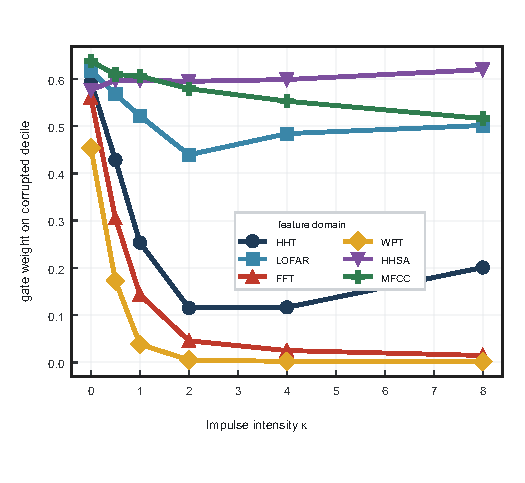
\includegraphics[width=\linewidth]{figures/fig2a.pdf}
  \end{minipage}\hfill%
  \begin{minipage}[t]{0.318\textwidth}
    \centering
    \fontsize{7.5}{8.5}\selectfont (b)\\[-0.45em]
        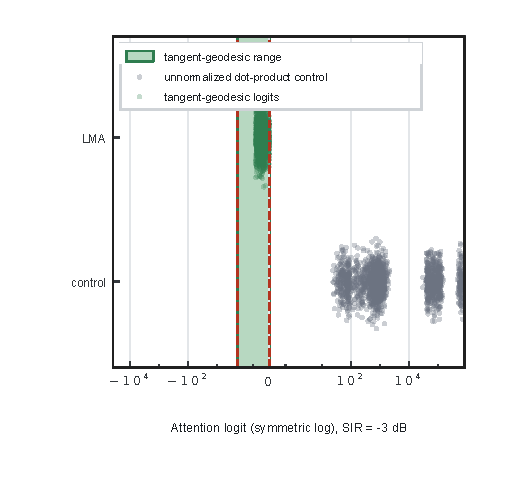
\includegraphics[width=\linewidth]{figures/fig2b.pdf}
  \end{minipage}\hfill%
  \begin{minipage}[t]{0.318\textwidth}
    \centering
    \fontsize{7.5}{8.5}\selectfont (c)\\[-0.45em]
        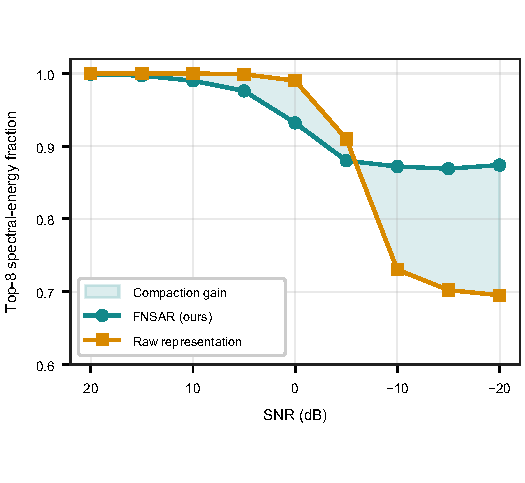
\includegraphics[width=\linewidth]{figures/fig2c.pdf}
  \end{minipage}
  \caption{Controlled mechanism diagnostics assembled from separately extracted vector panels. (a) GST reliability across descriptor domains versus impulse intensity. (b) Tangent-metric LMA logits and an unnormalized dot-product control at SIR $=-3$ dB. (c) Top-$8$ spectral-energy fraction before and after FNSAR.}
  \label{fig:mechanisms}
\end{figure*}

The compound condition is the harder mechanism test because all three failures act simultaneously. Figure~\ref{fig:compound-geometry} shows two complementary UMAP diagnostics from the controlled study. At the sample level, compound degradation disperses and overlaps class embeddings; after the complete model, the plotted clusters become more compact and separated. At the descriptor level, corruption disturbs the relative organization of the six domains, while reliability weighting and tangent projection tighten the domain clusters. Together, the two views show how the proposed reliability-conditioned geometry organizes both class-level and descriptor-level representations under compound degradation.

\begin{figure}[t]
  \centering
  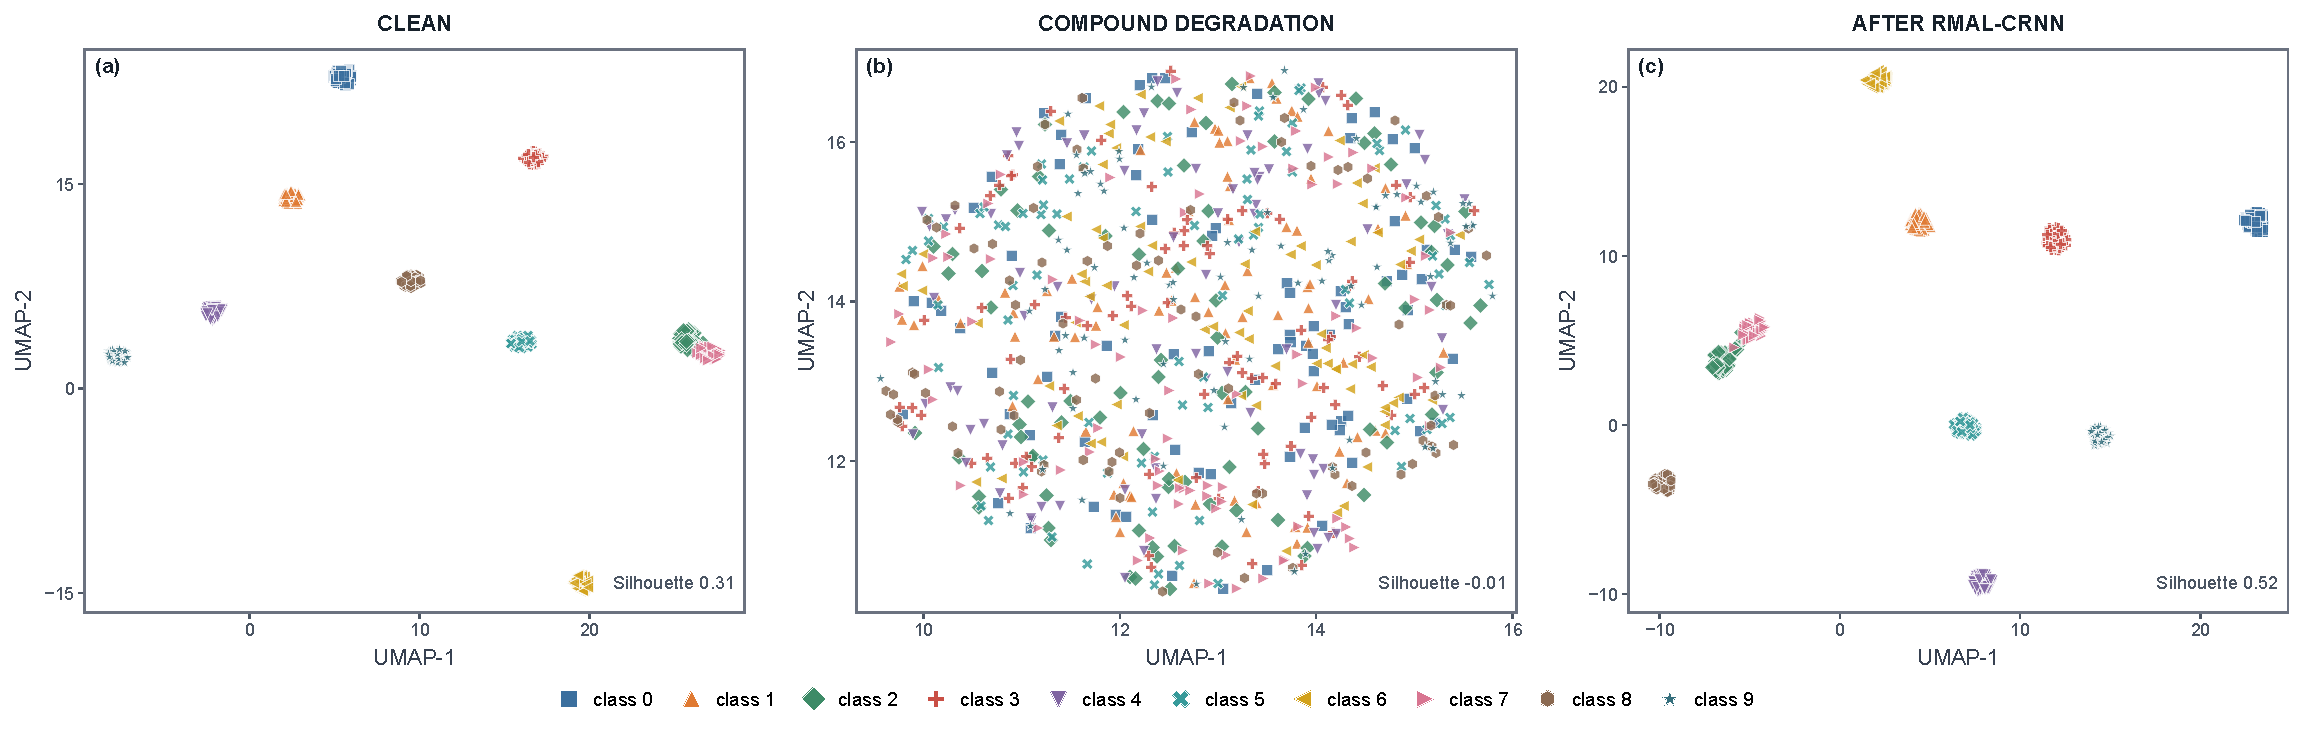
\includegraphics[width=\linewidth]{figures/fig3a.pdf}\\[0.72em]
  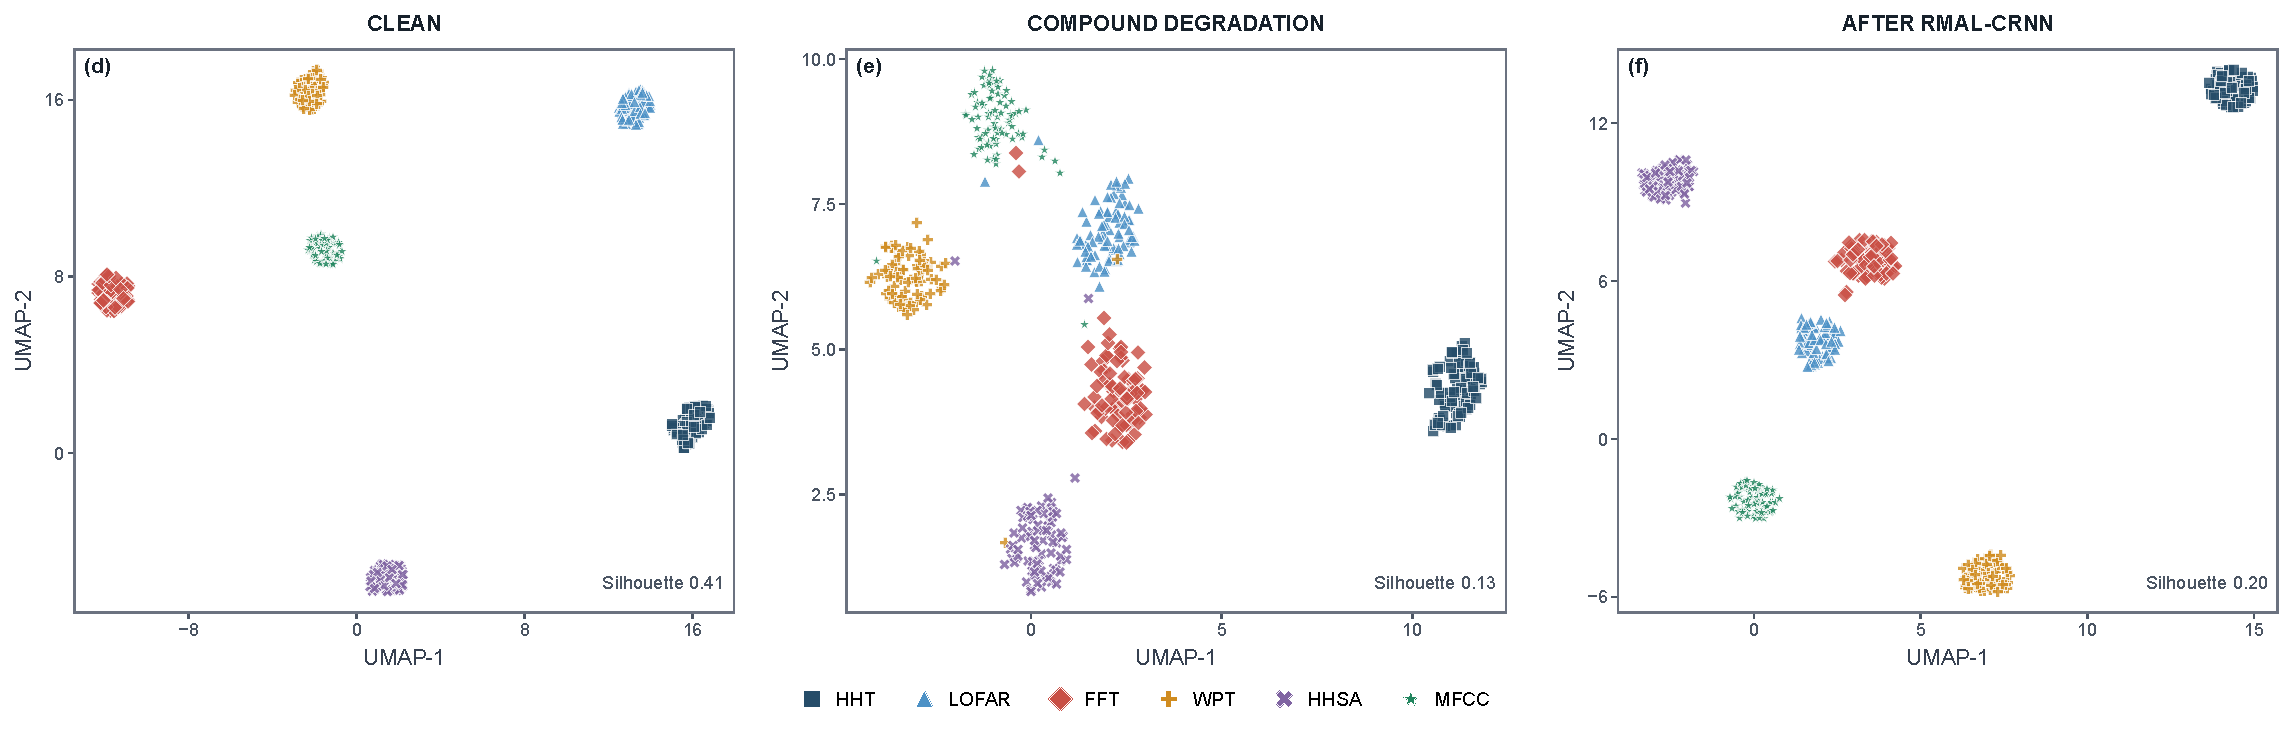
\includegraphics[width=\linewidth]{figures/fig3b.pdf}
  \caption{UMAP diagnostics under compound degradation. Top: clean, corrupted, and RMAL-CRNN sample embeddings. Bottom: clean, corrupted, and reliability-conditioned product-tangent descriptor embeddings.}
  \label{fig:compound-geometry}
\end{figure}

\subsection{Q2: Robust Classification}
Table~\ref{tab:comparison} compares sequence, convolutional, attention, forecasting, and manifold-oriented models on both benchmarks. RMAL-CRNN has the highest listed mean throughout. On Kielce it reaches $86.30\%$ and $93.88\%$ at $-5$ and $0$ dB, exceeding the strongest baseline by $2.27$ and $3.03$ points. On Glasgow it reaches $81.18\%$ at $0$ dB versus $74.28\%$ for CRNN, and remains ahead at lower SNRs. The consistent gains across both released benchmarks demonstrate the value of reliability-conditioned relation learning for low-SNR acoustic recognition.

\begin{table*}[t]
\caption{Accuracy across SNRs (\%, mean $\pm$ sample standard deviation) on the ten-class Kielce UAV-model benchmark (a) and the eight-class Glasgow/ACSAC~2022 acoustic-identity benchmark (b).}
\label{tab:comparison}
\centering
\small
\setlength{\tabcolsep}{2pt}
\textbf{(a) Kielce, ten classes}\par\vspace{0.25em}
\begin{tabular}{@{}lcccc@{}}
\toprule
Model (literature index) & $-5$ dB & $0$ dB & $5$ dB & $10$ dB\\
\midrule
MAtt-A \citep{pan2022matt} & $69.65{\pm}1.07$ & $80.33{\pm}1.43$ & $84.50{\pm}1.41$ & $88.65{\pm}1.17$\\
InceptionTime \citep{fawaz2020inceptiontime} & $78.90{\pm}0.79$ & $86.30{\pm}0.42$ & $90.75{\pm}0.70$ & $94.65{\pm}0.50$\\
CNN-Transformer \citep{vaswani2017attention} & $79.55{\pm}0.97$ & $86.83{\pm}0.48$ & $91.23{\pm}0.70$ & $93.85{\pm}0.45$\\
CRNN \citep{cakir2017crnn} & $80.80{\pm}0.82$ & $87.15{\pm}0.33$ & $91.80{\pm}0.34$ & $94.68{\pm}0.64$\\
SEResNet1D \citep{hu2020senet} & $81.98{\pm}0.49$ & $89.28{\pm}0.13$ & $92.73{\pm}0.52$ & $95.78{\pm}0.46$\\
TCN \citep{bai2018tcn} & $83.70{\pm}1.22$ & $90.85{\pm}0.49$ & $93.15{\pm}0.19$ & $96.28{\pm}0.39$\\
TimeMixer++ \citep{wang2025timemixerpp} & $84.03{\pm}1.21$ & $89.48{\pm}0.78$ & $93.68{\pm}0.60$ & $96.68{\pm}0.49$\\
MambaSL \citep{jung2026mambasl} & $82.53{\pm}1.15$ & $89.28{\pm}1.07$ & $93.20{\pm}0.18$ & $95.98{\pm}0.36$\\
RMAL-CRNN (ours) & \textbf{$86.30{\pm}0.29$} & \textbf{$93.88{\pm}0.36$} & \textbf{$96.08{\pm}0.35$} & \textbf{$97.48{\pm}0.51$}\\
\bottomrule
\end{tabular}
\par\vspace{0.65em}
\textbf{(b) Glasgow/ACSAC 2022 \citep{diao2022drone}, eight classes}\par\vspace{0.25em}
\begin{tabular}{@{}lcccc@{}}
\toprule
Model (literature index) & $-15$ dB & $-10$ dB & $-5$ dB & $0$ dB\\
\midrule
MAtt-A \citep{pan2022matt} & $30.35{\pm}1.38$ & $41.68{\pm}1.78$ & $54.43{\pm}1.23$ & $65.12{\pm}0.41$\\
InceptionTime \citep{fawaz2020inceptiontime} & $38.90{\pm}1.27$ & $54.25{\pm}1.51$ & $66.85{\pm}0.72$ & $75.02{\pm}1.31$\\
CNN-Transformer \citep{vaswani2017attention} & $38.32{\pm}0.34$ & $55.10{\pm}0.57$ & $69.12{\pm}0.66$ & $78.53{\pm}0.40$\\
CRNN \citep{cakir2017crnn} & $35.35{\pm}1.15$ & $51.38{\pm}1.02$ & $66.50{\pm}1.75$ & $74.28{\pm}0.62$\\
SEResNet1D \citep{hu2020senet} & $40.75{\pm}0.19$ & $56.12{\pm}0.88$ & $69.38{\pm}1.04$ & $78.50{\pm}1.13$\\
SPDNet \citep{huang2017spdnet} & $34.62{\pm}0.21$ & $46.03{\pm}1.45$ & $61.85{\pm}1.45$ & $70.88{\pm}2.43$\\
TCN \citep{bai2018tcn} & $36.35{\pm}1.31$ & $50.30{\pm}0.52$ & $65.05{\pm}1.50$ & $74.95{\pm}0.58$\\
BiLSTM \citep{graves2005bilstm} & $36.42{\pm}0.57$ & $50.68{\pm}1.84$ & $65.83{\pm}1.14$ & $73.95{\pm}0.44$\\
RMAL-CRNN (ours) & \textbf{$45.28{\pm}1.21$} & \textbf{$62.70{\pm}0.91$} & \textbf{$74.10{\pm}0.88$} & \textbf{$81.18{\pm}1.64$}\\
\bottomrule
\end{tabular}
\end{table*}

Figure~\ref{fig:confusion} complements the aggregate results with class-wise behavior at $0$ dB. In the reported run, HHT and HHSA exhibit broader off-diagonal errors, and direct concatenation does not recover the strongest individual-domain structure. RMAL-CRNN produces the most concentrated diagonal among the displayed matrices. This panel provides a class-wise view alongside the aggregate paired analysis below.

\begin{figure}[t]
  \centering
  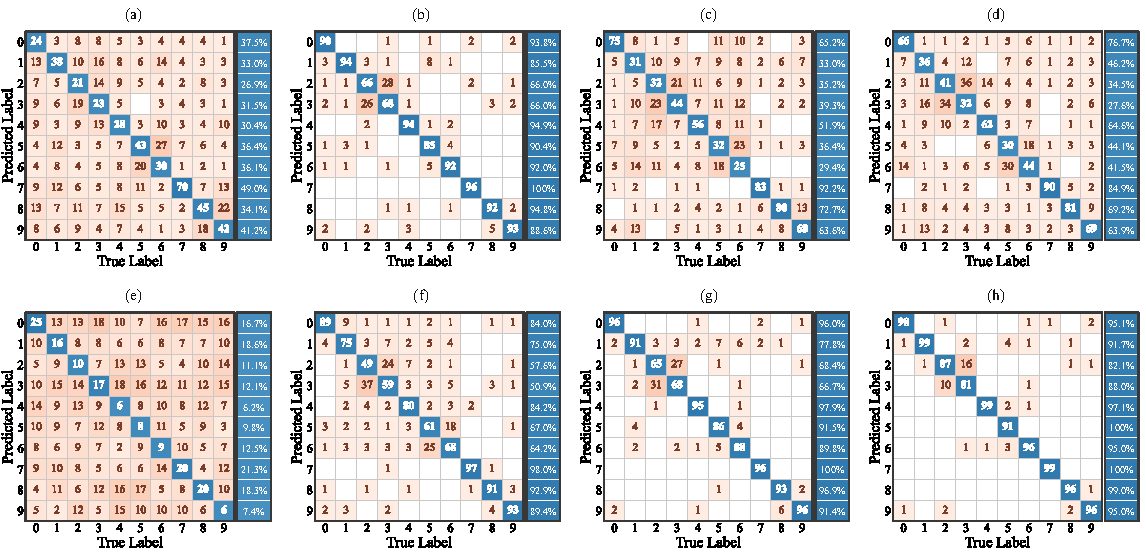
\includegraphics[width=0.98\linewidth]{figures/fig4.pdf}
  \caption{Confusion matrices at $0$ dB: (a) HHT, (b) LOFAR, (c) FFT, (d) WPT, (e) HHSA, (f) MFCC, (g) descriptor concatenation, and (h) RMAL-CRNN. Cell entries are counts; right-margin percentages are row-wise precision for each predicted class.}
  \label{fig:confusion}
\end{figure}

\subsection{Q3: Component Necessity}
We remove one operation at a time with fixed data and training settings. Exact full-model parameter counts, including the CRNN classifier, are given in Appendix~\ref{app:implementation}. Table~\ref{tab:ablation} reports losses of $1.41$, $1.50$, and $1.80$ points without FNSAR, LMA, and GST, and $6.96$ points against the CRNN control. Changes use unrounded paired run differences, explaining the apparent $0.01$ discrepancy from subtracting the rounded RMA-CRNN means. The ablation results use multiple random seeds, and the paired statistics summarize these runs.

The reported paired tests provide a second summary of the ablation runs: all listed $95\%$ confidence intervals for the complete-minus-control difference have positive lower bounds, and the reported Holm--Bonferroni-adjusted $p$-values are below $0.05$. Together with the component ablations, these results identify reliability estimation, tangent-metric relation learning, and sparse temporal affinity as complementary sources of the observed gain.

\begin{table}[t]
\caption{Structural ablations at $0$ dB (\%, mean $\pm$ standard deviation).}
\label{tab:ablation}
\centering
\small
\begin{tabular}{@{}llcc@{}}
\toprule
Variant & Composition & Accuracy & Change\\
\midrule
RMAL-CRNN & GST + LMA + FNSAR & $93.89{\pm}0.33$ & --\\
RMA-CRNN & GST + LMA & $92.47{\pm}0.49$ & $-1.41$\\
RL-CRNN & GST + FNSAR & $92.39{\pm}0.52$ & $-1.50$\\
MAL-CRNN & LMA + FNSAR & $92.09{\pm}0.38$ & $-1.80$\\
CRNN & baseline & $86.93{\pm}0.35$ & $-6.96$\\
\bottomrule
\end{tabular}
\end{table}
